\documentclass[12pt, twoside]{article}
\usepackage[francais]{babel}
\usepackage[T1]{fontenc}
\usepackage[latin1]{inputenc}
\usepackage[left=5mm, right=5mm, top=5mm, bottom=5mm]{geometry}
\usepackage{float}
\usepackage{graphicx}
\usepackage{array}
\usepackage{multirow}
\usepackage{amsmath,amssymb,mathrsfs}
\usepackage{soul}
\usepackage{textcomp}
\usepackage{eurosym}
 \usepackage{variations}
\usepackage{tabvar}

\pagestyle{empty}
\begin{document}


\section*{\center{Correction devoir maison 7}}

\bigskip

\bigskip

\bigskip

\begin{tabular}{cc}
\begin{minipage}{6cm}
\ul{Exercice 1}:

\enskip

autres noms pour $\widehat{GBH}$: \thinspace 
$\widehat{HBG}$ 

$\widehat{yBx}$ \quad  $\widehat{xBy}$ \quad  $\widehat{GBI}$ \quad 
$\widehat{IBG}$ 

$\widehat{JBI}$ \quad  $\widehat{IBJ}$ \quad  $\widehat{JBH}$ \quad
$\widehat{HBJ}$


\enskip

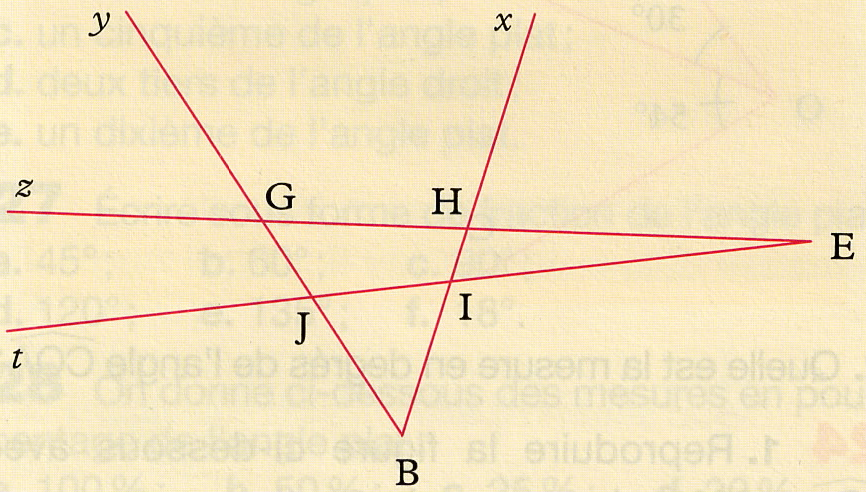
\includegraphics[width=6cm]{images/ex1.png}
\end{minipage}










&
\begin{minipage}{13cm}

\qquad \quad 
\ul{Exercice 2}:

\enskip

\qquad \quad 
\begin{tabular}{|c|c|c|c|}
\hline


angle & nom de l'angle & 
\begin{minipage}{3,1cm}
aigu, obtus, droit ou plat
\end{minipage} &
\begin{minipage}{3,1cm}
mesure de l'angle (au rapporteur)
\end{minipage}

\\

\hline

1 & $\widehat{xAz}$ & aigu &  45� \\

\hline

4 & $\widehat{pRt}$ & obtus &  94� \\

\hline

5 & $\widehat{aEb}$ & aigu & 83� \\

\hline

6 & $\widehat{rOs}$ & obtus & 176� \\

\hline

3 & $\widehat{mXn}$ & droit & 90� \\

\hline

2 & $\widehat{eDy}$ & obtus & 134� \\

\hline


\end{tabular}
\end{minipage}
\end{tabular}


\bigskip

\bigskip

\ul{Exercice 3}:

Les points C, D et E sont align�s donc $\widehat{CDE}$=180�. D'apr�s les
codages, on sait que $\widehat{NDO}=\widehat{ODM}=$30�.

\enskip

$\widehat{CDE}=\widehat{CDM}+\widehat{MDO}+\widehat{ODN}+\widehat{NDE}$
donc $\widehat{NDE}$=180-(50+30+30)=180-110=70 

\enskip

$\widehat{NDE}$ mesure 70�.


\bigskip

\bigskip



\ul{Exercice 4}:


\enskip

 U, L et M sont align�s signifie que l'angle \ldots
\ldots est \ldots \ldots(c'est-�-dire $\widehat{\ldots \ldots}=$ \ldots�).

\enskip

$\widehat{ULM}=\widehat{ULC}+\widehat{CLD}+\widehat{DLM}$= 40 + 43 + 56
=179� $\neq$ 180�

\enskip

$\widehat{ULM}$ n'est pas un angle \ldots \ldots \ldots donc les points U, L et
M ne sont pas \ldots \ldots.



\bigskip

\bigskip

\ul{Exercice 6}:


\enskip




3. $\widehat{CBA}= \widehat{CBD}+ \widehat{DBA}$

donc $\widehat{CBD}= 180-60=120$�

\enskip

5. $\widehat{ABD}= 120$�  

\enskip

[BE) est la bissectrice de l'angle $\widehat{ABD}$ donc l' angle
$\widehat{EBD}$ mesure 60�.

\enskip

$\widehat{EBD}=\widehat{CBD}=60$� donc la demi-droite [BD) partage
l'angle $\widehat{EBC}$ en deux angles m�me mesure. 

Cela signifie que [BD) est la
bissectrice de l'angle $\widehat{EBC}$.


\end{document}
